\chapter[Transient resonances in EMRIs]{Transient resonances in extreme-mass-ratio inspirals}\label{ch:resonances}

There are three fundamental frequencies $\Omega_k$ ($k=\{r,\,\theta,\,\phi\}$) describing bound orbits in the Kerr spacetime, corresponding to libration-type motions in the radial and polar directions, and a rotation in the azimuthal direction. At infinity, all three fundamental frequencies coincide, tending to the Keplerian frequency, but elsewhere they become distinct, with $\Omega_r < \Omega_\theta < \Omega_\phi$. Frequencies evaluated using different time coordinates can be related to each other by multiplicative factors, and so it follows that there is a well-defined notion of \textit{ratios} of frequencies. An orbit is said to exhibit a resonance when the ratio of any two frequencies is a rational number.

Resonances involving the $\phi$ frequency cannot affect the local dynamics of an EMRI system due to the axisymmetry of the Kerr spacetime. Any dynamical quantity $q$ must depend only on $r$ and $\theta$ along the worldline, and so may be Fourier expanded in coordinate time according to
\begin{equation}
\label{eq:res-dynamical-exp}
q(t) = \sum_{n,m} q_{nm} \exp\left[-\iu\left( n\Omega_r + m\Omega_\theta \right)t\right],
\end{equation}
with no dependence on $\Omega_\phi$. However, it has been shown that both $\theta\phi$-resonances \citep{hirata_resonant_2011} and $r\phi$-resonances \citep{van_de_meent_resonantly_2014} can lead to extrinsic effects. The GWs from such systems are not emitted isotropically and the imbalance produces a kick velocity that is, in some cases, sufficient to eject the central BH from its host.

We shall be interested in systems that exhibit $r\theta$-resonances, such that
\begin{equation}
\label{eq:res-def}
\zeta \equiv \frac{\Omega_r}{\Omega_\theta} = \frac{n_\theta}{n_r},
\end{equation}
where $n_\theta$ and $n_r$ are integers with no common multiples; we shall refer to such a system as being in a $n_\theta$:$n_r$ resonance. The effects of these resonances were first studied by \citet{flanagan_transient_2012}, who calculated the non-perturbative `jumps' in the orbital parameters as the evolution of an EMRI passes through a resonance. These occur because the two-frequency Fourier expansion in \eqnref{res-dynamical-exp} becomes invalid on resonance and should be replaced by a single-frequency series. This results in enhanced or diminished GW fluxes on resonance. \Citet{gair_resonances_2012} considered two toy models for this behaviour, differing in whether the phase or the frequency components should be continuous across the resonance. It is not fully understood which of these models provides the better description.

It is possible for resonances to capture an orbit and thus become long-lived, but such sustained resonances are likely to be very rare and so unobservable with typical GW detectors \citep{van_de_meent_conditions_2014}. In contrast, short-lived transient resonances have been found to be near-ubiquitous in EMRI systems \citep{ruangsri_census_2014} and are located in the strong-field regime close to the SMBH \citep{brink_astrophysics_2015, brink_orbital_2015}, where GW emission is significant. Typical variations of GW fluxes due to resonances are of the order of a few percent \citep{flanagan_resonantly_2014}. We extend this existing body of work by considering the effect of transient resonances on the detectability of EMRIs using GWs. However, we first discuss our method of including resonances within an evolution scheme, and provide an exploration of the relevant properties of resonances.

\section{Evolution scheme}
\label{sec:EMRI-evolution-scheme}
For generic EMRIs, there are two timescales of interest \citep{hinderer_two-timescale_2008}: the \emph{fast} orbital motion, related to the fundamental frequencies $\sim1/\Omega$, and the \emph{slow} inspiral, related to the change in fundamental frequencies $\sim\Omega/\dot{\Omega}$, where an overdot denotes a derivative with respect to coordinate time $t$. This makes it ideally suited to the method of osculating elements~\citep{gair_forced_2011}: on short timescales, we analyse the unperturbed system resulting in geodesic motion; while the long-term evolution is described by a sequence of instantaneous geodesics. We require, at each instant in time, that the chosen geodesic matches the true position and velocity of the particle. This amounts to a specific choice of the orbital shape parameters and the positional elements, collectively referred to as \emph{osculating elements} and denoted by $I^A$. For our evolution, we choose to consider $I^A = \{p(t),\,e(t),\,\cos\iota(t),\,\psi_0(t),\chi_0(t),\phi_0(t)\}$, making explicit the variation with time. These quantities are defined in \secref{kerr-geodesic}.

Given forced motion in a background spacetime, the acceleration
\begin{equation}
f^\alpha = \difftwo{x^\alpha}{\tau} + \Gamma^\alpha_{\beta\gamma}\diff{x^\beta}{\tau}\diff{x^\gamma}{\tau},
\end{equation}
can be used to calculate the evolution of the osculating elements $\dot{I}^A(f^\alpha)$. The specific equations for Kerr are derived by \citet{gair_forced_2011}. Using these equations and the notation of \secref{kerr-geodesic}, the resulting system of differential equations to be solved takes the form
\begin{subequations}
\label{eq:kerr-osc-el-ev}
\begin{align}
\label{eq:kerr-osc-el-ev-I}
\diff{I^A}{t} &= \dot{I}^A\left(\psi(t),\,\chi(t);\,I^A\right),\quad &I^A(0) &= I^A_0,\\
\diff{\psi}{t} &= \dot{\lambda} \frac{p}{r^2 e} \sqrt{\frac{R(r)}{1-\cos^2\psi}} - \diff{\psi_0}{t},\quad &\psi(0) &= \psi_0(0),\\
\diff{\chi}{t} &= \dot{\lambda} \sqrt{\frac{(1-\cos^2\theta_\mathrm{inc}\cos^2\chi)\Theta(\theta)}{\cos^2\theta_\mathrm{inc}\sin^2\chi}} - \diff{\chi_0}{t},\quad &\chi(0) &= \chi_0(0),
\end{align}
\end{subequations}
where $\dot{\lambda} = (\dd \tau/\dd t)/\Sigma$ is the coordinate-time derivative of Mino time, which can be evaluated using \eqnref{kerr-geodesics-t}. If desired, we may also compute $\tau$ and $\phi$ by evolving them directly according to \eqnref{kerr-geodesics}. We perform the integration numerically using the standard fourth order Runge--Kutta method. We choose a step size equal to the minimum of $5\,\mathrm{s}$ and $2\pi/(8\Omega_r)$, which ensures that the fast orbital motion is modelled sufficiently accurately.\footnote{In \chapref{effect-resonances}, we compute the GWs from these systems. The fixed maximum step size of $5\,\mathrm{s}$ is chosen to ensure that the high frequency cut-off in the emitted GWs is above the most sensitive frequency of typical detectors.}

%This formalism can be used to study many kinds of small perturbations, including the effect of a distant massive object (that might be expected if an EMRI occurs during a galactic merger), the role of internal structure or spin of the compact object, and deviations of the metric from GR.

\subsection{Gravitational self-force model}
We are interested in using this evolution scheme to study the perturbation arising from the curvature generated by the particle itself. We cannot use established adiabatic techniques to describe the inspiral as the assumptions made are incompatible with transient $r\theta$-resonances. Instead, we choose to work directly with the gravitational self-force, using the same PN approximation as \citet{flanagan_transient_2012}. For comparison, \citet{flanagan_resonantly_2014} use a Teukolsky equation calculation of resonant GW fluxes.

The self-force model we adopt uses the first-order PN terms of the dissipative self-force formulated by \citet{flanagan_evolution_2007} and the conservative force formulated by \citet{iyer_post-newtonian_1993}, and \citet{kidder_coalescing_1995}. Since only the first PN terms are used, this prescription can only be of limited validity in strong fields. Both pieces of the self-force are computed assuming that the spin is small: the dissipative piece contains terms to $\order{a^2}$ and the conservative piece to $\order{a}$. This is less than ideal for high spins. While this approximate self-force is not perfect, it should serve as a guide for the behaviour of the full self-force, allowing us to assess the qualitative impact of resonances on EMRI detection.

\subsection{Adiabatic averaging}
\label{sec:res-ad-averaging}
We can study the effect of resonances by comparing an adiabatic evolution with an instantaneous self-force evolution. Using adiabatic results from the literature is useful to test the efficacy of the self-force model, but is not ideal in this case. Differences between the evolutions may arise due to the different approaches being taken, rather than as a result of transient resonances. We therefore, instead, construct an appropriate adiabatic trajectory using our self-force model, by explicitly averaging the fluxes\footnote{We use the term flux here to denote the rate of change of orbital parameters. For the case of $E$ and $L_z$, this is equivalent to (minus) the physical flux of those quantities carried by the emitted GWs, but a similar physical interpretation does not exist for the other parameters.} of our osculating elements over the $r\theta$ $2$-torus. Computing this average is trivial  if the quantity is parameterised in terms of the generalised action-angle variables $\{q_r, q_\theta\}$,
\begin{equation}
\left\langle \diff{X}{\lambda}\right\rangle_{q_r,\,q_\theta} = \frac{1}{(2\pi)^2}\intd{0}{2\pi}{\intd{0}{2\pi}{\diff{X}{\lambda}}{q_r}}{q_\theta}.
\end{equation}
However, we are using $\psi$ and $\chi$, as these are simpler to evolve. Furthermore, using the osculating elements formalism, we compute instantaneous coordinate-time fluxes $\dot{X}$, not Mino-time fluxes. Changing variables gives an average of \citep{drasco_computing_2005}
\begin{align}
\left\langle \diff{X}{\lambda}\right\rangle_{q_r,\,q_\theta} = {} & \frac{1}{\Lambda_r \Lambda_\theta}\intd{0}{2\pi}{\intd{0}{2\pi}{\left(\diff{\psi}{t}\right)^{-1} \left(\diff{\chi}{t}\right)^{-1} \left(\diff{t}{\lambda}\right)^{-2} \diff{X}{\lambda}}{\psi}}{\chi} \nonumber\\
 = {} & \frac{1}{\Lambda_r \Lambda_\theta}\intd{0}{2\pi}{\intd{0}{2\pi}{\left(\diff{\psi}{t}\right)^{-1} \left(\diff{\chi}{t}\right)^{-1} \left(\diff{t}{\lambda}\right)^{-1} \dot{X}}{\psi}}{\chi}.
\label{eq:2torus-average}
\end{align}
This average describes the Mino-time rate of change of the quantity $X$ over an orbit. To convert to a coordinate-time flux of the averaged quantity, we simply divide by the period $\Gamma$, defining
\begin{equation}
\dot{\left\langle X\right\rangle}_{q_r,\,q_\theta} = \frac{1}{\Gamma}\left\langle \diff{X}{\lambda}\right\rangle_{q_r,\,q_\theta}.
\end{equation}
It is convenient to calculate $\Gamma$ as
\begin{equation}
\Gamma = \left\langle \diff{t}{\lambda}\right\rangle_{q_r,\,q_\theta},
\end{equation}
using \eqnref{2torus-average}, as this allows us to eliminate $\Lambda_r$ and $\Lambda_\theta$ from the calculation.

We compute these integrals using a $N\times M$ grid of $(\psi,\chi)$ values and employing a Newton--Cotes approximation in each dimension. Specifically we take $N = M = 300$, and approximate each integral by
\begin{align}
\intd{x_1}{x_n}{f(x)}{x} \approx \delta x \bigg(&\frac{17}{48}f(x_1) + \frac{59}{48}f(x_2) + \frac{43}{48}f(x_3) + \frac{49}{48}f(x_4)\nonumber\\
& + \left\{f(x_5) + \ldots + f(x_{n-4})\right\}\nonumber\\
& + \frac{49}{48}f(x_{n-3}) + \frac{43}{48}f(x_{n-2}) + \frac{59}{48}f(x_{n-1}) +  \frac{17}{48}f(x_n)\bigg),
\end{align}
where $x_i = x_1 + (i-1)\delta x$, $x_1 = 0$, and $\delta x = 2\pi / (N-1)$. This procedure requires $\mathcal{O}(10^5)$ separate evaluations of the derivatives at each time-step of an evolution, and so is computationally expensive to perform. The adiabatic derivatives vary on much longer timescales than the orbital motion, and so in practice, we can make use of interpolation. We calculate the adiabatic derivatives, as above, at three points in the inspiral spaced by $\dd t/\eta$ where $\dd t$ is the orbital time-step. When the system is close to the central point, we use a quadratic fit to estimate the adiabatic derivatives. Once the system evolves close to one of the boundaries, we update the interpolation points, taking the closest boundary to be the new central point.

%We compute these integrals using a grid of $(\psi,\chi)$ values: we split each integral into $25$ equal segments and then evaluate each of those segments using Boole's rule, which is a specific case of the Newton-Cotes method\footnote{Newton-Cotes formulae for approximating integrals are derived by fitting a polynomial to the integrand using equally spaced intermediate values. The trapezium rule and Simpson's rule are well-known examples, which use linear and quadratic fitting functions respectively. Boole's rule uses a quartic polynomial.}. The integral of $f(x)$ between $x_1$ and $x_5$ is approximated by
%\begin{equation}
%\intd{x_1}{x_5}{f(x)}{x} \approx \frac{2 h}{45}\left( 7f(x_1) + 32 f(x_2) + 12 f(x_3) + 32 f(x_4) + 7f(x_5) \right),
%\end{equation}
%where $x_i = x_1 + (i-1)h$. This procedure requires $101\times 101$ separate evaluations of the derivatives at each time-step of an evolution, and so is computationally expensive to perform. The adiabatic derivatives vary on much longer timescales than the orbital motion, so in practice, we can make use of interpolation. We calculate the adiabatic derivatives, as above, at three points in the inspiral spaced by $dt/\sqrt{\eta}$ where $dt$ is the orbital time-step\footnote{The evolution timescale of an EMRI $\sim 1/\eta$ and so we could space the interpolation points further apart; we choose $1/\sqrt{\eta}$ instead to be on the cautious side.}. When the system is close to the central point, we use a quadratic fit to estimate the adiabatic derivatives. Once the system evolves close to one of the boundaries, we update the interpolation points, taking the closest boundary to be the new central point.

To demonstrate the approach, we calculate the instantaneous evolution and the 2-torus-averaged adiabatic evolution over $2$ years for a set of initial parameters chosen to avoid any significant resonances. Specifically, we choose: the mass of the compact object $\mu = 10 M_{\odot}$; the mass ratio $\eta = 3\times 10^{-6}$; the spin of the central BH $a=0.95$; the orbital shape parameters $p=7.5$, $e=0.7$ and $\cos \iota = 0.5$; and the redshift of the source $z=0.204$ (corresponding to $1\;\mathrm{Gpc}$ in our chosen $\Lambda$CDM cosmology, used in \secref{EMRI-detectability}). The remaining intrinsic (the initial phases $\psi_0$ and $\chi_0$) and extrinsic parameters are set to arbitrary values. The resulting evolutions of $E$, $L_z$ and $Q$ are shown in \figref{good-traj}, where it can be seen that the adiabatic evolution closely matches the instantaneous evolution on longer inspiral timescales. The inset plots show the start of the evolution, on a timescale associated with the orbital motion; the 2-torus averaging explicitly smoothes out the visible structure on this scale.

%The resulting averaged fluxes successfully describe the leading-order secular evolution of the trajectory, as illustrated in \figref{good-traj} by an EMRI that does not encounter any significant resonances.

\begin{figure}[htbp]
\centering
\subfloat{\includegraphics[width=0.7\textwidth]{good_traj_E}}\\
\subfloat{\includegraphics[width=0.7\textwidth]{good_traj_Lz}}\\
\subfloat{\includegraphics[width=0.7\textwidth]{good_traj_Q}}
\caption{\label{fig:good-traj}The evolution of the orbital parameters $E$ (upper figure), $L_z$ (middle) and $Q$ (lower) under the instantaneous (solid line) and adiabatic (dashed) models for an illustrative EMRI system that does not encounter any significant resonances. The inset plots show the behaviour on short timescales, where the fast orbital oscillations can be seen.}
\end{figure}

%\subsection{Quasi-adiabatic averaging}
%The effect of resonances must be completely contained within the pieces of the self-force left after subtraction of the $2$-torus-averaged pieces, $\hat{X}\equiv X-\langle X\rangle_{q_r,\,q_\theta}$. The adiabatic evolution, which contains only a single $2$-torus-averaged forcing term, will therefore not be affected by the occurence of any transient resonances. Resonances still occur as the fundamental frequencies vary, but as the system passes through each resonance, there is no additional effect on the evolution of the system.

%Comparing instantaneous and adiabatic evolutions may be a useful exercise to calibrate and verify adiabatic models that can be generated cheaply; however it cannot be used to distinguish between dephasing effects arising from resonances and those arising from conservative corrections to the phase variables, as both are explicitly eliminated from the adiabatic prescription. We therefore take a slightly different approach, comparing the instantaneous evolution with a quasi-adiabatic evolution, generated by averaging the full available self-force over the $2$-torus, rather than just averaging the term $G_\alpha^{(1)}$.

%To be specific, returning to the action-angle formalism, we write \eqnref{EMRI-AAsf} as
%\begin{subequations}
%\label{eq:res-AAsf}
%\begin{align}
%\diff{q_\alpha}{\tau} = {} & \omega_\alpha(\boldsymbol{J}) + \eta \langle g_\alpha\rangle_{q_r,\,q_\theta}(\boldsymbol{J}) + \eta \hat{g}_\alpha(q_r,q_\theta,\boldsymbol{J}), \\
%\diff{J_\alpha}{\tau} = {} & \eta \langle G_\alpha\rangle_{q_r,\,q_\theta}(\boldsymbol{J}) + \eta \hat{G}_\alpha(q_r,q_\theta,\boldsymbol{J}),
%\end{align}
%\end{subequations}
%where $g_\alpha$ and $G_\alpha$ encapsulate all our knowledge about the self-force and may in principle contain contributions from sub-leading terms in the mass-ratio expansion. The quasi-adiabatic evolution is then obtained by dropping the terms containing $\hat{g}_\alpha$ and $\hat{G}_\alpha$. For ease of notation, we shall drop the \emph{quasi-} identifier; all subsequent references to an ``adiabatic evolution'' in fact refer to a ``quasi-adiabatic evolution''.


\section{Properties of transient resonances}
%The combination of an instantaneous self-force evolution and a 2-torus-averaged adiabatic evolution allows us to systematically study the effect of transient resonances on EMRIs over the course of an inspiral.% Before approaching this problem, we first investigate the properties of the resonances themselves.

\subsection{Location of resonances}
\label{sec:res-location}
In order to efficiently study transient resonances, it is essential to know where they occur in parameter space. A system exhibiting a $n_\theta$:$n_r$ resonance must obey the constraint
\begin{equation}
\label{eq:res-condition}
\Omega \equiv n_r \Omega_r(p,e,\cos\iota;a) - n_\theta \Omega_\theta(p,e,\cos\iota;a) = 0,
\end{equation}
where we have made explicit the dependence of the frequencies on $a$. The frequencies depend on the orbital shape parameters via elliptic integrals and so cannot be explicitly inverted. We instead adopt a numerical root-finding algorithm to calculate the value of $p$ such that the resonance condition holds. The mapping from the orbital shape parameters to the orbital frequencies is not one-to-one; there exist isofrequency pairings where two different sets of parameters result in the same frequencies \citep{warburton_isofrequency_2013}. One of these pairs is located very close to the SMBH in a region where we expect the orbits to be evolving very quickly. We therefore focus on the more distant resonances, as these are still within the strong-field regime of the spacetime, but are more long-lived.

\begin{figure}[htbp]
\centering
\subfloat{\includegraphics[width=\textwidth]{resplane_a}}\\
\vspace{20pt}
\subfloat{\includegraphics[width=\textwidth]{resplane_res}}
\caption{\label{fig:res-resplane}Resonance surfaces, defined by \eqnref{res-condition}, in the orbital shape parameter space $\{p,\,e,\,\cos\iota\}$. The upper figure demonstrates the 2:3 resonance, at different values of the SMBH spin, while the lower figure fixes the spin at $a=0.95$ and depicts the surfaces for different resonances.}
\end{figure}

\Figref{res-resplane} shows the resonance surfaces in the orbital shape parameter space, for different values of the spin, and for different resonances. The surfaces are closely approximated by planes and so it is natural to consider whether some simple functional form can predict their location. For a given resonance ratio $\zeta$, the semi-latus rectum can be found using
\begin{equation}
\label{eq:res-approx-p}
p(e,\cos\iota;a,\zeta) \simeq A\frac{1 + B e + D \cos\iota}{1 - C\exp(e)},
\end{equation}
where the coefficients are given by
\begin{subequations}
\begin{align} 
A(a,\zeta) \simeq {} & a_0\frac{1 + a_1\zeta - a_2 \zeta^2 - a_3 \zeta a^2}{1 + a_4\zeta - (1 + a_4)\zeta^2}, \\
B(a,\zeta) \simeq {} & b_0(1 - b_1\zeta)\exp(-b_2\zeta)(1 - b_3 a), \\
C(a,\zeta) \simeq {} & c_0, \\
D(a,\zeta) \simeq {} & d_0\left[1 - \exp(a)\right]\left[1 - d_1\exp(\zeta)\right].
\end{align}
\end{subequations}

We generate resonance location data for all possible resonances with $2 \leq n_r \leq 7$, as well as $\zeta = 9/10$, $19/20$, $49/50$ and $99/100$, for SMBH spins between $0.01 \leq a \leq 0.999$, eccentricities in the range $0.01 \leq e \leq 0.99$ and inclinations with $-0.999999 \leq \cos\iota \leq 0.999999$. We then fit this data to the functional form in \eqnref{res-approx-p}, obtaining optimised parameters
\begin{equation}
\begin{array}{lll}
a_0 = 5.9854, & a_1 = 3.4116, & a_2 = 0.9253,\\
a_3 = 0.1959, & a_4 = 4.8846, & b_0 = 0.7692,\\
b_1 = 1.4752, & b_2 = 1.4861, & b_3 = 0.5974,\\
c_0 = 0.02332, & d_0 = 0.7968, & d_1 = 0.3115.
\end{array}
\end{equation}
This gives an approximation to the true resonant semi-latus rectum, which provides a convenient starting point for numerical root-finding algorithms. Our $12$-parameter model might be expected to overfit the data. However, we note that a simple quadratic expansion in the four variables requires $15$ free parameters and yet gives a worse fit to the data. In \figref{res-reserror}, we show the fractional error in $p$ for our fit, marginalising over $e$ and $\cos\iota$ by considering both the maximal value and the root-mean-square (RMS). Typical errors are a few percent, while the largest relative errors occur for highly spinning BHs as $\zeta\rightarrow 0$. In these cases, the value of $p$ is small such that the absolute error is less than $1$.

\begin{figure}[htbp]
\centering
\subfloat{\includegraphics[width=0.92\textwidth]{reserror_max}}\\
\subfloat{\includegraphics[width=0.92\textwidth]{reserror_rms}}
\caption{\label{fig:res-reserror}The relative error in $p$ of our approximation to the location of resonances. At each value of $a$ and $\zeta$, we compute the absolute maximum (upper figure) and RMS (lower) error over $e$ and $\cos\iota$. Lighter shades correspond to larger values of the error.}
\end{figure}

%The approximant given by \eqnref{res-approx-p} should not be taken as an exact location for any given resonance, but instead as an indication of the region of parameter space in which resonances occur, providing a convenient starting point for numerical root-finding algorithms.


\subsection{Resonance timescales}
\label{sec:res-timescales}
Resonant phenomena occur on timescales intermediate to the orbital timescale $\tau_\mathrm{orb} \sim 2\pi/\Omega_k$ and the evolution timescale $\tau_\mathrm{ev} \sim \zeta/\dot{\zeta} \sim \mathcal{O}(\tau_\mathrm{orb}/\eta)$. We can describe them by considering the phase-space precession inherent to non-resonant orbits but absent for resonant trajectories. We define the precession timescale
\begin{equation}
\tau_\mathrm{pres}(t) = \frac{2\pi}{|\Omega(t)|},
\end{equation}
where $\Omega(t)$ is defined by \eqnref{res-condition} and $t$ is the coordinate time of an EMRI evolution, taken to be zero on resonance. This is a measure of how long a particular orbit takes to come close to every point within the $r\theta$ 2-torus. This timescale is infinite exactly on resonance and decreases as the orbit evolves away. A suitable resonance timescale $\tau_\mathrm{res}$ can then be determined by considering the time at which the orbit has had sufficient opportunity to significantly precess. This is given by
\begin{align}
\tau_\mathrm{res} = \tau_\mathrm{pres}(\tau_\mathrm{res}) = \frac{2\pi}{|\Omega(\tau_\mathrm{res})|}.
\end{align}
Taylor expanding $\Omega(t)$ about resonance at $t=0$ and taking an adiabatic average of $\dot{\Omega}$ as we are mainly interested in the long-term secular evolution here, we obtain
\begin{align}
\tau_\mathrm{res} \simeq \frac{2\pi}{\left|\left\langle\dot{\Omega}(0)\right\rangle_{q_r,\,q_\theta}\right| \tau_\mathrm{res}},
\end{align}
which can be rearranged to give
\begin{align}
\label{eq:res-timescale}
\tau_\mathrm{res} = \left[ \frac{2\pi}{\left|\left\langle\dot{\Omega}(0)\right\rangle_{q_r,\,q_\theta}\right|} \right]^{1/2}.
\end{align}
In terms of the mass ratio, we see that the resonance timescale $\tau_\mathrm{res} \sim \mathcal{O}(\eta^{-1/2}\tau_\mathrm{orb}) \sim \mathcal{O}(\eta^{1/2}\tau_\mathrm{ev})$ and so acts as a bridge between the other two timescales.

\begin{figure}[htbp]
\centering
\subfloat{\includegraphics[width=0.33\textwidth]{geotraj_1}}
\subfloat{\includegraphics[width=0.33\textwidth]{geotraj_2}}
\subfloat{\includegraphics[width=0.33\textwidth]{geotraj_3}}
\caption{\label{fig:res-geotraj}Three geodesic trajectories for an EMRI with SMBH mass $M = 1.2\times10^6 M_\odot$, spin $a=0.95$, compact object mass $\mu = 12 M_\odot$, eccentricity $e = 0.7$, and inclination $\cos\iota = 0.2$. The left-hand plot has a semi-latus rectum $p = 9.398644$, which corresponds to a 2:3 resonance, with a resonance timescale $\tau_\mathrm{res}\approx0.02\,\mathrm{yrs}$. The central and right-hand plots have initial conditions given by an inspiralling evolution $\tau_\mathrm{res}/2$ and $\tau_\mathrm{res}$ after resonance respectively. Each geodesic is shown for a finite time $\tau_\mathrm{res}/2$ only.}
\end{figure}

We demonstrate these results by considering geodesic orbits nearby to a resonance. \Figref{res-geotraj} shows three `snapshot' orbits, each evolved for the same amount of time (in this case, we evolve for half a resonance timescale). The first trajectory is exactly on a 2:3 resonance and it can be seen that no precession takes place. The second and third trajectories have initial conditions that correspond with an inspiralling orbit at a time $T$ after passing through the 2:3 resonance (we take $T$ to be $\tau_\mathrm{res}/2$ and $\tau_\mathrm{res}$ for the two cases respectively). The resonance has an impact on the evolution for approximately a resonance timescale $\tau_\mathrm{res}$, after which the 2-torus is quickly filled by the trajectory, validating the adiabatic approach.

\subsection{Resonant flux enhancements}
Evolving through a region that does not contain a significant resonance,\footnote{A significant resonance noticeably affects the evolution of the EMRI. We intuitively expect only low-order resonances to be significant; this can be seen by considering the resonance timescale. High-order resonances have large values of $n_r + n_\theta$ and so have smaller values of $\tau_\mathrm{res}$, from \eqnref{res-timescale}. The resonance is not significant unless $\tau_\mathrm{res} > \tau_\mathrm{orb}$.} the trajectory quickly fills the $r\theta$ 2-torus and we may approximate the motion by replacing $\dd I^A/\dd t$ with $\langle\dd I^A/\dd t\rangle_{q_r,\,q_\theta}$, producing the adiabatic evolution. However, evolving through a resonance, this average is not a good approximation. With respect to the adiabatic case, there is an enhancement (or decrement) of the fluxes that depends on the relative phase of $q_r$ and $q_\theta$. After crossing the resonance region, we therefore expect to find different orbital parameters to those of an equivalent adiabatic trajectory. This difference is given by \citet{flanagan_transient_2012} as
\begin{equation}
\label{eq:res-jump}
\Delta I^A_\mathrm{jump} = \eta\sum_{s \neq 0} F^A_s(\boldsymbol{I}) \left[ \frac{2\pi}{\left|s\left\langle\dot{\Omega}\right\rangle_{q_r,\,q_\theta}\right|} \right]^{1/2} \exp\left[\iu (s q_0 + \frac{\pi}{4}\sgn s\dot{\Omega})\right],
\end{equation}
where $q_0$ is the adiabatic phase associated with the frequency $\Omega$ on resonance, and $F^A_s$ is the Fourier component of the self-force, defined such that
\begin{equation}
\diff{I^A}{t} = \eta\sum_s F^A_s(\boldsymbol{I})\exp(\iu s q).
\end{equation}
This result can be derived using matched asymptotic expansions, and can be understood as the product of the forcing function on resonance with the resonance timescale.

We use two equivalent methods to numerically demonstrate the effects of \eqnref{res-jump}. First, we evolve orbits through resonances and compute the jumps directly by considering the orbital parameters before and after the resonance. Second, we calculate the resonant fluxes along fixed geodesics.

\subsubsection{Orbital parameter jumps}
\label{sec:res-orb-jumps}
We consider a collection of EMRIs a short time before crossing the 2:3 resonance. At this point, we are not interested in the emitted GWs and so only the intrinsic parameters are relevant. For each system, we choose a mass ratio $\eta = 3\times 10^{-6}$, eccentricity $e=0.7$, and inclination $\cos\iota = 0.2$. We then vary the spin to take values $a = j/10$ for $j=[1,9]$, as well as $a = \{0.01,\,0.95,\,0.99\}$. We also vary the initial radial phase, choosing $\psi_0$ to take 50 equally spaced values between $0$ and $2\pi$. We keep $\chi_0 = 0$ fixed, and so this should span the full range of $q_0$ in \eqnref{res-jump}, enabling us to estimate the magnitude of $\Delta I^A_\mathrm{jump}$.

We evolve each of these systems through the resonance using the instantaneous self-force model and the 2-torus-averaged adiabatic model, as detailed in \secref{EMRI-evolution-scheme}. When the system encounters the 2:3 resonance, the instantaneous evolution undergoes a rapid change in the orbital parameters with respect to the adiabatic evolution, as shown for the orbital energy in \figref{res-jump-calc}. To extract the magnitude of the jump from the trajectory data, we first must account for the fast orbital oscillations as well as ensure that we include the full effect of the resonance, while minimising any contributions resulting from other sources.

To achieve this, we isolate spans of data away from the resonance. Specifically, we consider data that lies within five and ten resonance timescales away. For both the pre- and post-resonance regions, we compute $\Delta I^A(t) \equiv I^A_{\mathrm{inst}}(t) - I^A_\mathrm{ad}(t)$ for each of the orbital parameters. We then identify the most-horizontal straight lines that bound the data, which give an approximation to the behaviour of the fast orbital oscillations. The dashed green and yellow lines in \figref{res-jump-calc} demonstrate this bounding procedure.

\begin{figure}[htbp]
\centering
\includegraphics[width=0.92\textwidth]{res_jump_calc}
\caption{\label{fig:res-jump-calc}The difference in energy between the instantaneous model and an adiabatic model, scaled by the magnitude of the 2:3 resonance jump. The thickness of the (blue) line is due to the fast orbital oscillations, which cannot be seen on this scale. The dashed green (yellow) lines show the bounding fits to the data before (after) the resonance, used to numerically estimate the size of the jump. The dotted red line indicates the computed size of the jump. The time axis is centred on the 2:3 resonance and is scaled by the resonance timescale.}
\end{figure}

To estimate the size of the jump $\Delta I^A_{\mathrm{jump}}$, we extrapolate the bounding lines to the resonance time and calculate the difference between the pre- and post-resonance values, quoting the final result as the average of that obtained using the upper and lower limits. This allows us to take into account any linear drift in $\Delta I^A(t)$ that can occur over the resonance timescale due to the inaccuracy of the adiabatic approximation. %In addition, by using information from both the upper and lower limits, we can veto jump calculations that appear erroneous\footnote{This is not a concern for the current systems being studied, but in \chapref{effect-resonances}, we study resonances that occur very near to plunge and do not follow the typical behavior described here.}. 
Our numerically computed jump appears to suitably describe the behaviour through resonance, as shown by the red dotted line in \figref{res-jump-calc}.

We compute the 2:3 resonance jump in this manner for each EMRI system in our collection. The absolute size of the resonance jump is often not particularly useful, especially when comparing different systems. Instead, we can express it relative to the adiabatic change expected across the resonance. Using the resonance timescale from \eqnref{res-timescale} to set the length of the resonance, we compute the ratio for each orbital parameter as
\begin{equation}
\label{eq:res-jump-ratio}
\frac{\Delta I^A_\mathrm{jump}}{\left\langle\Delta I^A\right\rangle} = \frac{\Delta I^A_\mathrm{jump}}{I^A_\mathrm{ad}(t_\mathrm{res} + \tau_\mathrm{res}/2)-I^A_\mathrm{ad}(t_\mathrm{res} - \tau_\mathrm{res}/2)} \approx \frac{\Delta I^A_\mathrm{jump}}{\dot{I}^A_\mathrm{ad}(t_\mathrm{res})\tau_\mathrm{res}}.
\end{equation}
As a function of $\psi_0$, we expect these jumps to be oscillatory, as a result of \eqnref{res-jump}. In \figref{res-jump-vs-psi0}, we display the computed relative resonance jumps in energy, for three of our chosen values of the BH spin. The oscillations are sinusoidal, with a spin-dependent amplitude $|\Delta I^A_\mathrm{jump}|$ that can be calculated by taking half the difference between the maximum and minimum values. %The phase difference between the cases is due to the offset between $\psi_0$ and the phase on resonance $q_0$, which is different for each value of $a$ due to the different inspiral rates.
We plot the relative magnitudes as a function of BH spin in \figref{res-jump-vs-a}; typical jumps are of the order of a percent. The negative values indicate that the adiabatic evolution has a negative derivative.

\begin{figure}[htbp]
\centering
\includegraphics[width=0.92\textwidth]{res_jump_vs_psi0}
\caption{\label{fig:res-jump-vs-psi0}The relative jump in energy, calculated using \eqnref{res-jump-ratio}, due to crossing the 2:3 resonance, as a function of the initial radial phase $\psi_0$, which acts as a proxy for the relative phase on resonance $q_0$. The jumps are shown for three values of the BH spin, $a = 0.1$ (blue), $0.5$ (gold) and $0.95$ (green) with thicker lines representing higher values of spin.}
\end{figure}

\begin{figure}[htbp]
\centering
\subfloat{\includegraphics[width=0.7\textwidth]{res_jump_E_vs_a}}\\
\subfloat{\includegraphics[width=0.7\textwidth]{res_jump_Lz_vs_a}}\\
\subfloat{\includegraphics[width=0.7\textwidth]{res_jump_Q_vs_a}}
\caption{\label{fig:res-jump-vs-a}The magnitude of the relative jump in energy (upper figure), angular momentum (middle) and Carter constant (lower), due to crossing the 2:3 resonance, as a function of BH spin $a$. Data is shown for the jump method (solid line), discussed in \secref{res-orb-jumps}, and for the flux method (dashed), discussed in \secref{res-geo-fluxes}.}
\end{figure}

This method of studying the resonance jumps is conceptually straightforward, since we are directly measuring the quantity of interest. However, for jumps that are much smaller than the width of the fast orbital oscillations, it can be difficult to extract the jump magnitude from the data. This is especially true when resonances occur close to plunge. There is an alternative way to compute the relative resonance jumps without explicitly evolving the system, which we now discuss.

\subsubsection{Fluxes on resonant geodesics}
\label{sec:res-geo-fluxes}
We have previously evolved generic Kerr inspirals by solving the differential system given by \eqnref{kerr-osc-el-ev}. We now seek to evolve a different, but closely-related, system representing a fixed geodesic trajectory, while still considering the effects of the self-force. We replace \eqnref{kerr-osc-el-ev-I} with
\begin{subequations}
\begin{align}
\diff{P^A}{t} &= \dot{I}^A\left(\psi(t),\,\chi(t);\,I^A\right),\quad &P^A(0) &= 0,\\
\diff{I^A}{t} &= 0,\quad &I^A(0) &= I^A_0,
\end{align}
\end{subequations}
where $P^A$ are auxilliary variables used to compute the integrated fluxes along an orbit but that have no impact on the evolution. We are interested in the secular accumulation of the osculating elements arising from the self-force during a resonance, and how this depends on the relative phase between the $r$ and $\theta$ motions. In order to average out the fast orbital motion, we compute the long-time average,
\begin{equation}
\label{eq:res-geo-flux-diff}
\dot{I}^A_\mathrm{inst} \equiv \left\langle \dot{P}^A \right\rangle_T = \lim_{T\rightarrow\infty} \frac{P^A(T)}{T},
\end{equation}
for each osculating element. For non-resonant geodesics, this quantity will depend only on the orbital shape parameters, but for resonant orbits there will be an additional dependence on the initial phase difference $\psi_0 - \chi_0$ (as a proxy for $q_0$).

We consider a selection of different orbital shape parameters corresponding to low-order transient resonances and calculate $\dot{I}^A_\mathrm{inst}$ for $50$ different initial phases $\psi_0$. In practice, to imitate the limiting behaviour at infinite times, we evolve for an integer number of cycles of both the radial and polar motions. Specifically, when considering a $n_\theta$:$n_r$ resonance, we take $T = 2\pi N n_\theta/\Omega_r = 2\pi N n_r/\Omega_\theta$ for some integer $N$. We have found that taking $N=5$ gives sufficiently accurate results.

Averaging $\dot{I}^A_\mathrm{inst}$ over the phase difference is equivalent to evolving under the adiabatic approximation. We can therefore estimate the relative orbital parameter jumps as
\begin{equation}
\label{eq:res-flux-enhnc}
\frac{|\Delta I^A_\mathrm{jump}|}{\left\langle\Delta I^A\right\rangle} \approx \frac{\max \dot{I}^A_\mathrm{inst} - \min \dot{I}^A_\mathrm{inst} }{2 \left\langle \dot{I}^A_\mathrm{inst} \right\rangle},
\end{equation}
where the maximum, minimum and mean values on the right-hand side are taken over $\psi_0$. Computing the resonant flux enhancements in this way for the same systems as discussed in \secref{res-orb-jumps}, we find good agreement between the two methods, as demonstrated in \figref{res-jump-vs-a}.

We now compute the $p$, $e$ and $\cos\iota$ flux enhancements for the 2:3 resonance with eccentricity $e=0.3$ and varying spin and inclination, displaying the results in \figref{res-flux-2to3-e03}. Typical enhancements in $p$ and $e$ are around $0.1\%$ and $1\%$ respectively, although they can be much smaller for orbits that are nearly equatorial. Intuitively the volume of space occupied by the $r\theta$ 2-torus of allowed motions is smaller for nearly equatorial orbits. Resonant orbits therefore come close to every allowed point, thus approximating a non-resonant orbit. We note that the signs of the values for $p$ and $e$ are negative, indicating that the adiabatic fluxes are both negative in this case.

It is expected that generic inclined orbits will adiabatically evolve to larger inclinations; in the weak-field, circular limit, the 2.5PN expansion is given up through $\mathcal{O}(e^2)$ by \citet{ganz_adiabatic_2007} as
\begin{align}
\left\langle \diff{\cos\iota}{t} \right\rangle = &-\frac{244}{15} \eta p^{-11/2} a (1-e^2)^{3/2} \sin^2\iota \bigg[\left(1+\frac{189}{61}e^2 \right)\nonumber\\
 &- \left(\frac{13}{244} + \frac{277}{244}e^2\right)a p^{-1/2}\cos\iota - \left(\frac{10461}{1708}+\frac{83723}{3416}e^2\right)p^{-1}\bigg],
\end{align}
indicating that to leading order, $\dot{\iota} \propto \sin\iota$ and is positive. This is confirmed for circular orbits in the strong-field regime using Teukolsky results \citep{hughes_evolution_2000}. In contrast, we observe regions of decreasing $\iota$ (increasing $\cos\iota$) for certain retrograde orbits; \figref{res-flux-2to3-e03} demonstrates such a region for eccentric orbits, but the behaviour is found to persist as $e\rightarrow 0$. We attribute this property of our evolutions to the specific self-force model being used, and note that the changes in inclination are small across the duration of a typical observation. Neglecting the anomalous retrograde orbits on the boundary between the regions of positive and negative adiabatic flux (such that the relative flux enhancements diverge), we find typical relative flux enhancements of $\cos\iota$ at the $1\%$ level.

\begin{figure}[htbp]
\centering
\subfloat{\includegraphics[width=0.7\textwidth]{res_flux_2to3_e03_p}}\\
\subfloat{\includegraphics[width=0.7\textwidth]{res_flux_2to3_e03_e}}\\
\subfloat{\includegraphics[width=0.7\textwidth]{res_flux_2to3_e03_cosi}}
\caption{\label{fig:res-flux-2to3-e03}Resonant flux enhancements for a 2:3 resonance with $e=0.3$ and for varying values of $a$ and $\cos\iota$. We display the enhancements for $p$ (upper figure), $e$ (middle) and $\cos\iota$ (lower). Larger enhancements are shaded darker, while negative and positive regions are blue and red respectively; the only positive values are found in the lower plot for the most retrograde systems.}
\end{figure}

Around marginally spinning BHs, as $a\rightarrow 0$, the absolute enhancements become symmetric with respect to $\cos\iota$, as expected. The smallest value of spin that we consider is $a=0.01$; for $a=0$ exactly, the enhancements vanish since we may always choose coordinates such that the motion lies in the equatorial plane, with no polar oscillations. We note that features at higher values of $a$ may not be physical due to the self-force model we are using.

\begin{figure}[htbp]
\centering
\subfloat{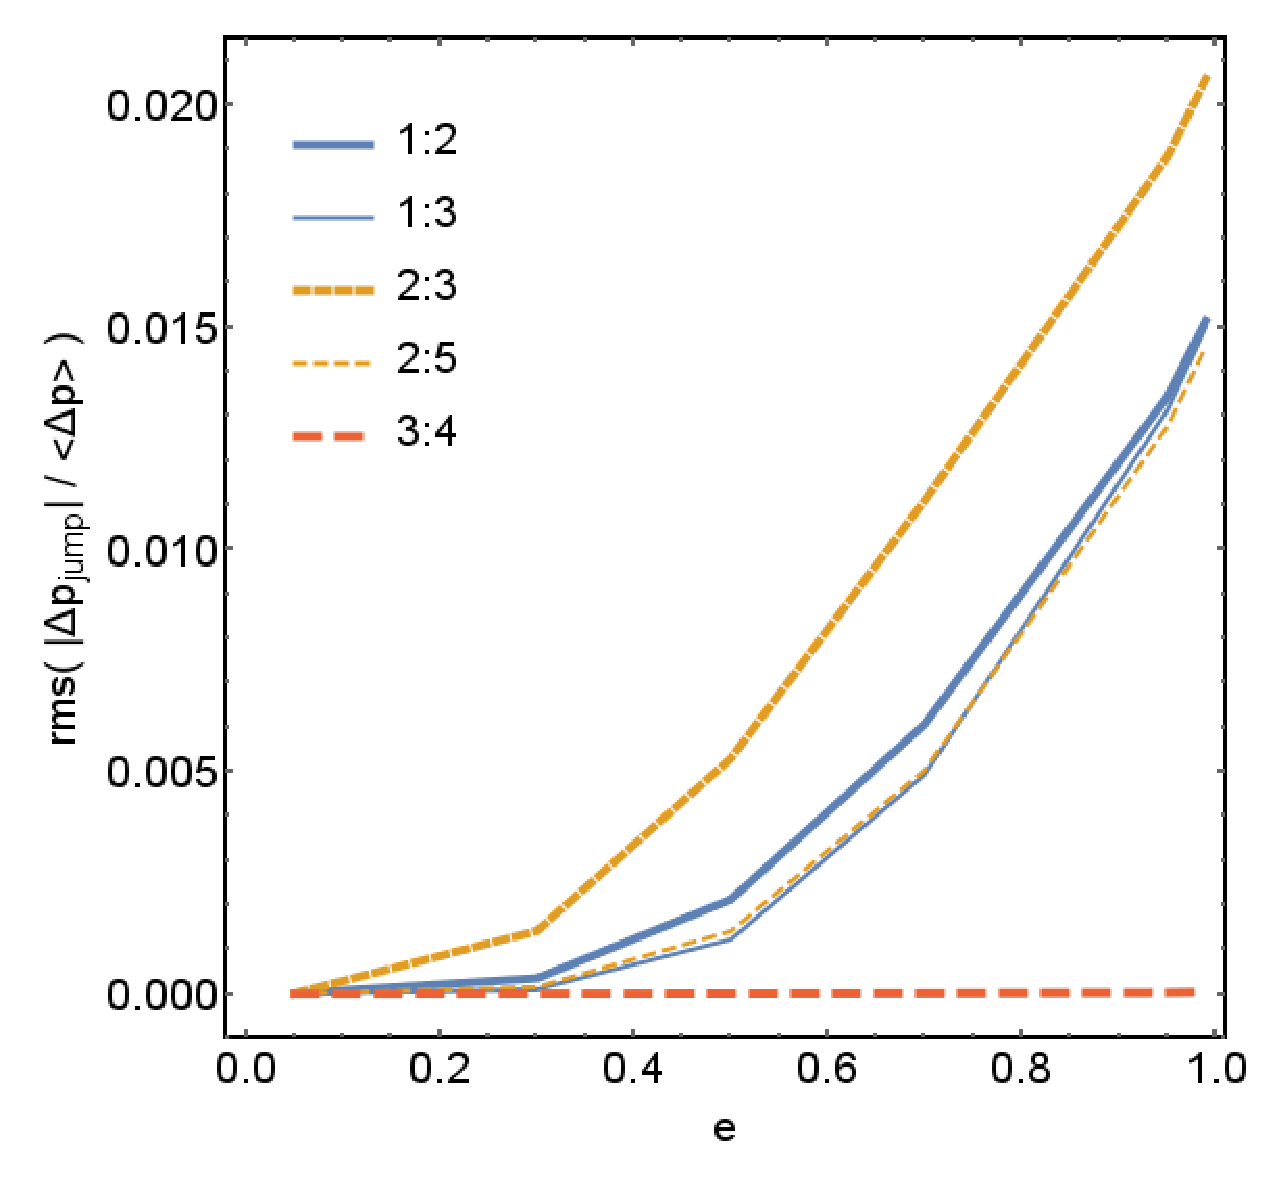
\includegraphics[width=0.5\textwidth]{res_flux_rms_p}}
\subfloat{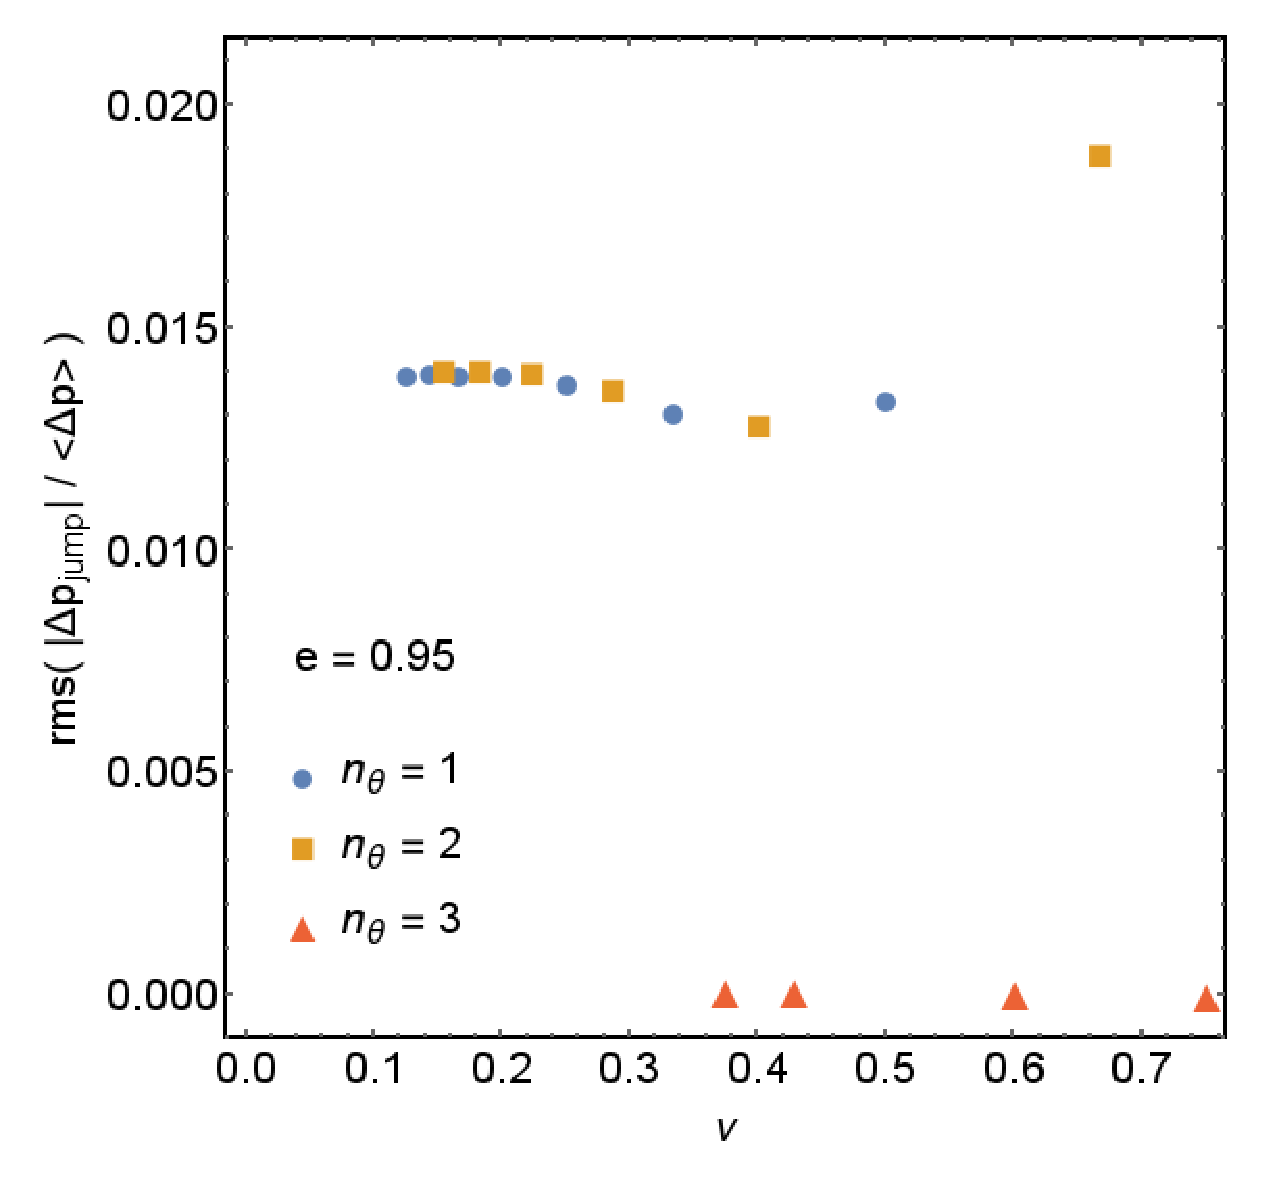
\includegraphics[width=0.5\textwidth]{res_flux_rms_p_e095}}
\caption{\label{fig:res-flux-rms-p}Relative flux enhancements of $p$, as a function of $e$ (left figure) and $\zeta$ (right), marginalised over $a$ and $\cos\iota$ by taking the root-mean-square of a grid of values. Resonances with $n_\theta = 1$ ($2$; $3$) are coloured blue (gold; red), use solid (short-dashed; long-dashed) lines and circular (square; triangular) points. The 2:3 resonance has the largest relative flux enhancement.}
\end{figure}

For the same reasoning that nearly-equatorial orbits show small flux enhancements, we expect nearly-circular orbits to exhibit similar behaviour due to the small volume of the $r\theta$ 2-torus. In figures \ref{fig:res-flux-rms-p}, \ref{fig:res-flux-rms-e} and \ref{fig:res-flux-rms-cosi}, we show the root-mean-square (over $a$ and $\cos\iota$) relative flux enhancements as a function of eccentricity, for a selection of low-order resonances. As expected, it is found that larger eccentricities give rise to larger resonant flux enhancements in general.

It is also interesting to consider the dependence on the resonance ratio $\zeta$. Fixing the eccentricity at $e=0.95$ to emphasise the variation, we compute the flux enhancements for different resonance ratios, shown in the right-hand plots of figures \ref{fig:res-flux-rms-p}, \ref{fig:res-flux-rms-e} and \ref{fig:res-flux-rms-cosi}, where we also highlight ratios arising from different values of $n_\theta$. We observe a clear relationship between the flux enhancement and $\zeta$ for all resonances with $n_\theta = 1$ or $2$, independent of which of those is considered. However, negligibly small flux enhancements are observed for systems with $n_\theta = 3$ or higher. This can be explained by the quadrupolar nature of GWs. A resonant trajectory averaged over time (and consequently $\phi$) takes $n_\theta$ (possibly repeated) values of $\theta$ at each radial turning point. Considering rings of matter at these coordinates, the dominant spherical harmonic describing the resultant mass distribution has $l=n_\theta$ (and $m=0$). Since GWs are generated by the quadrupole moment at leading order, the most significant resonant enhancements will arise from systems with $n_\theta = 2$. Due to the presence of higher harmonics, $n_\theta = 1$ systems also contribute strongly; it is perhaps more appropriate to treat $1$:$x$ resonances as \emph{de facto} $2$:$2x$ resonances, explaining the linked behaviour of the flux enhancements for $n_\theta = 1$ and $2$ systems.

\begin{figure}[htbp]
\centering
\subfloat{\includegraphics[width=0.5\textwidth]{res_flux_rms_e}}
\subfloat{\includegraphics[width=0.5\textwidth]{res_flux_rms_e_e095}}
\caption{\label{fig:res-flux-rms-e}Relative flux enhancements of $e$, as a function of $e$ (left figure) and $\zeta$ (right), rms marginalised over $a$ and $\cos\iota$. Considering the low-order resonances (those that have the longest duration), the 2:3 resonance is strongest. The divergence at $\zeta \approx 0.2$ is due to the adiabatic flux $\langle\Delta e\rangle \approx 0$ close to plunge.}
\end{figure}

As the lowest-order resonance with $n_\theta = 2$, the 2:3 resonance is the most significant, providing the largest flux enhancements over a prolonged time. The divergence in the relative flux enhancement of $e$ near $\zeta = 0.2$, observed in \figref{res-flux-rms-e}, is a consequence of the adiabatic behaviour. Under GW emission, eccentricities typically decrease, apart from for a short time prior to plunge where they slightly increase. There is hence some critical $p$ such that the adiabatic rate of change of $e$ vanishes. Higher-order resonances, with smaller $\zeta$, tend to occur closer to the central BH at smaller values of $p$, and so there is a corresponding critical value of $\zeta$ where $\langle\Delta e\rangle \approx 0$ and the relative flux enhancements diverge. However, the absolute flux enhancements remain small for these resonances, and so we do not expect them to influence the evolution any more than nearby resonances with much smaller relative enhancements.% Below the divergence, the adiabatic fluxes are positive.

\begin{figure}[htbp]
\centering
\subfloat{\includegraphics[width=0.5\textwidth]{res_flux_rms_cosi1}}
\subfloat{\includegraphics[width=0.5\textwidth]{res_flux_rms_cosi1_e095}}
\caption{\label{fig:res-flux-rms-cosi}Relative flux enhancements of $\cos\iota$, as a function of $e$ (left figure) and $\zeta$ (right), rms marginalised over $a$ and $\cos\iota$, restricted to prograde orbits only. The 2:3 resonance is the most significant.}
\end{figure}

The resonant enhancements to the fluxes of $E$, $L_z$ and $Q$ have been calculated previously using Teukolsky-based methods for a handful of systems by \citet{flanagan_resonantly_2014}. They consider the 1:2, 1:3, 2:3 and 3:4 resonances for EMRIs with $a=0.9$, either $e=0.3$ or $0.7$, and $\theta_\mathrm{inc} = 20\text{\textdegree}$ or $70$\textdegree. We compare our results to their published values (in their tables I--IV) in \figref{res-flux-FHR}. There is some qualitative agreement between the two approaches: more eccentric orbits give rise to larger enhancements; and the 3:4 resonance has a negligibly small enhancement. However, for the most significant 2:3 resonance, we typically predict larger orbital parameter jumps. Our results in \chapref{effect-resonances}, regarding the impact of resonances on a population of EMRIs, are therefore conservative predictions, as our model over-estimates the resonance effects.

\begin{figure}[htbp]
\centering
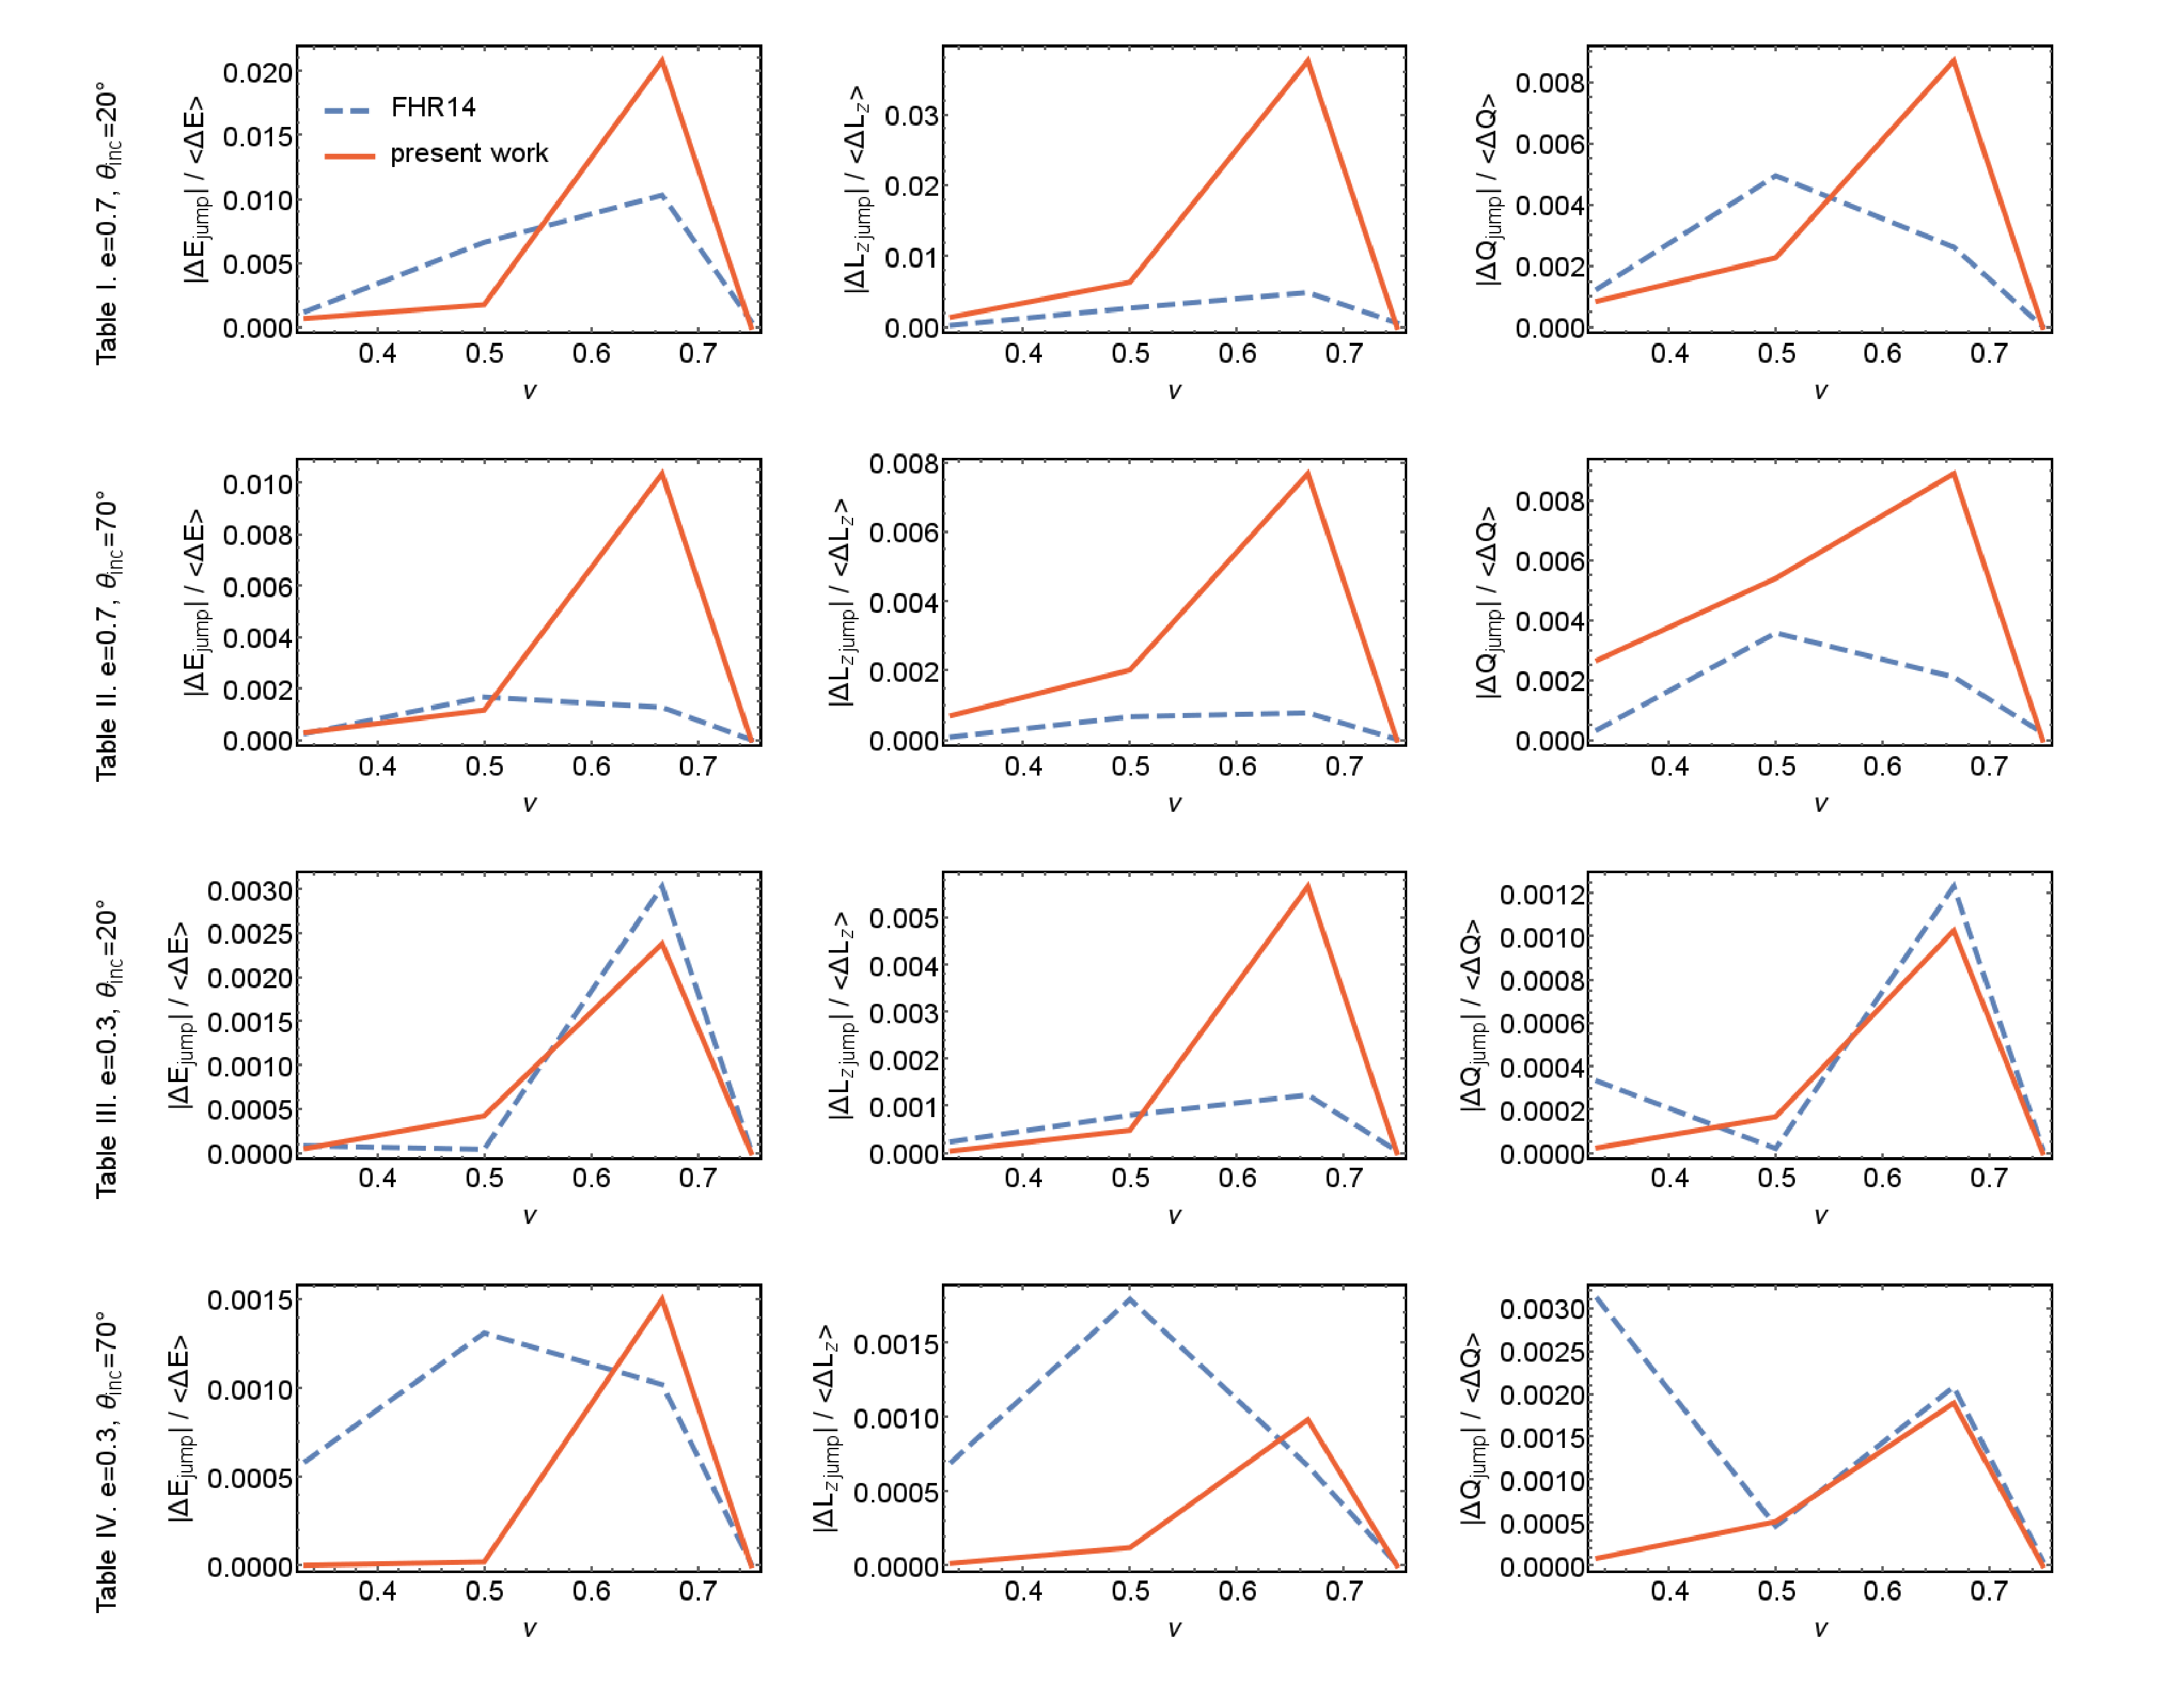
\includegraphics[width=\textwidth]{res_flux_FHR}
\caption{\label{fig:res-flux-FHR}Relative flux enhancements of $E$ (left column), $L_z$ (middle) and $Q$ (right) for resonance ratios corresponding to the 1:3, 1:2, 2:3 and 3:4 resonances. We show results as computed here with a solid red line, and results from \citet[FHR14]{flanagan_resonantly_2014} with a dashed blue line. Each row has a different eccentricity and inclination corresponding to tables I--IV in FHR14. All systems have $a=0.9$.}
\end{figure}

\section{Summary}
Transient resonances between the frequencies of motion in the $r$ and $\theta$ directions are expected to be nearly ubiquitous in observations of EMRI systems, and yet are unaccounted for by the standard adiabatic modelling techniques. These calculate the precession-averaged radiation fluxes using the Teukolsky equation and equate them to the rate of change of orbital parameters using balance arguments. However, on resonance, the orbit does not precess and fill the $r\theta$ 2-torus, and so this approach is insufficient to capture the full behaviour of the system. We instead use a gravitational self-force model to evolve EMRIs instantaneously, enabling us to study the properties of resonances.

We find the resonance surfaces in $p$--$e$--$\cos\iota$ space to be well-approximated by planes, with a fit given by \eqnref{res-approx-p}. This is sufficiently accurate to use as the starting point for numerical root-finding algorithms to determine the precise resonance location. As an EMRI evolves through a resonance, the rate of change of the orbital parameters is enhanced or diminished with respect to an adiabatic evolution, by an amount depending on the phase difference between the $r$ and $\theta$ motions. This leads to a rapid change in the parameters, often referred to as a jump. We compute the magnitude of this jump using two methods: analysing the phase space trajectory during an evolution to extract the jump directly; and calculating the flux enhancements while fixed on a resonant geodesic. Typical jumps are around $1\%$, and are greatest for the 2:3 resonance. There is a strong dependence on the eccentricity of the system, with more eccentric orbits experiencing much larger flux enhancements.

The magnitude of the orbital parameter jumps cannot tell us about the impact of resonances on GW observations of EMRIs. For that, we must calculate the emitted GWs from each system and study the loss in SNR that arises from using adiabatic templates.

